\documentclass[twocolumn,english]{scrartcl}
\usepackage{babel, fontspec, amsmath}
\usepackage{graphicx, float}
\usepackage{datetime2}
\setmainfont[Numbers=OldStyle]{Linux Libertine O}
\setkomafont{sectioning}{\rmfamily}
\title{Confocal Spectroscopy of gated WSe2 Bilayer}
\usepackage{graphicx, float}
\author{By God Himself}
\date{\DTMdate{2017-11-17}}
\begin{document}
\maketitle
\centering{Experiment performed on:}\\
\centering{\DTMdate{2017-9-22} -- \DTMdate{2017-10-6}}
\begin{tabular}{ll}
Parameter&Value\\
\hline\\
\end{tabular}
\begin{figure}[H]
\centering
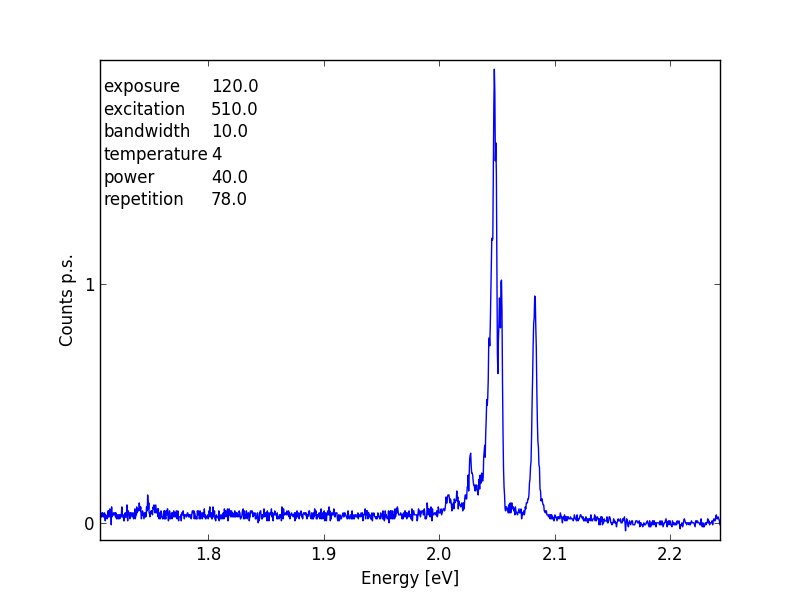
\includegraphics[width=0.45\textwidth]{WL-SCAN-01-hbn-WS2-hbn-SiO-40uW-510nm+-5nm-WLS-78MHz-120s-x41329y08629.png}
\caption{Filename:WL-SCAN-01-hbn-WS2-hbn-SiO-40uW-510nm+-5nm-WLS-78MHz-120s-x41329y08629.png}
\end{figure}
\begin{figure}[H]
\centering
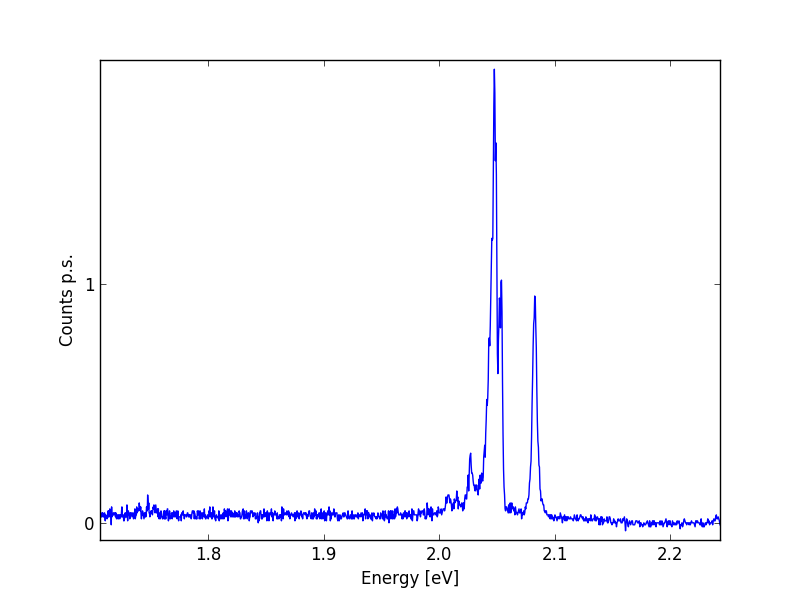
\includegraphics[width=0.45\textwidth]{Ex.png}
\caption{Filename:Ex.png}
\end{figure}
\begin{figure}[H]
\centering
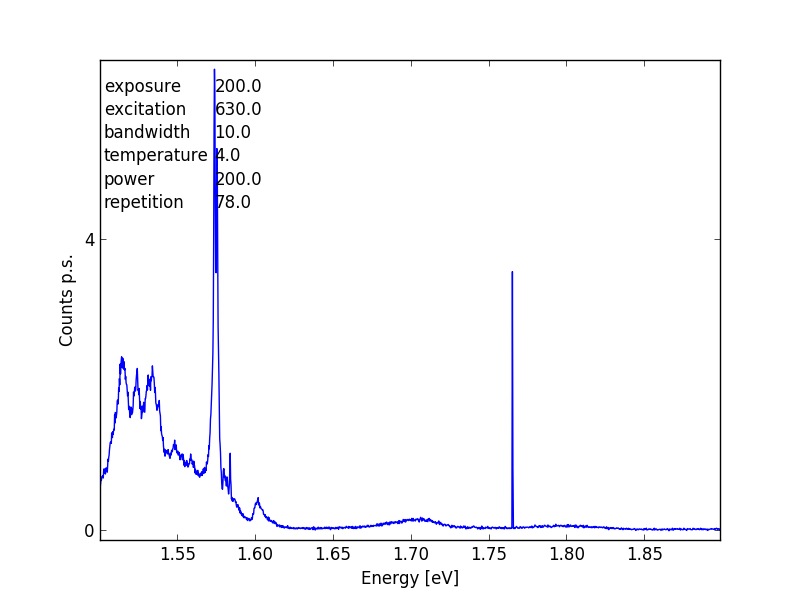
\includegraphics[width=0.45\textwidth]{GATE-08-hbn-WSe2-hbn-200uW-200s-630nm+-5nm-4K-nogate-78MHz-timetrace-0V-xm03081y22400_1.png}
\caption{Filename:GATE-08-hbn-WSe2-hbn-200uW-200s-630nm+-5nm-4K-nogate-78MHz-timetrace-0V-xm03081y22400\_1.png}
\end{figure}
\begin{figure}[H]
\centering
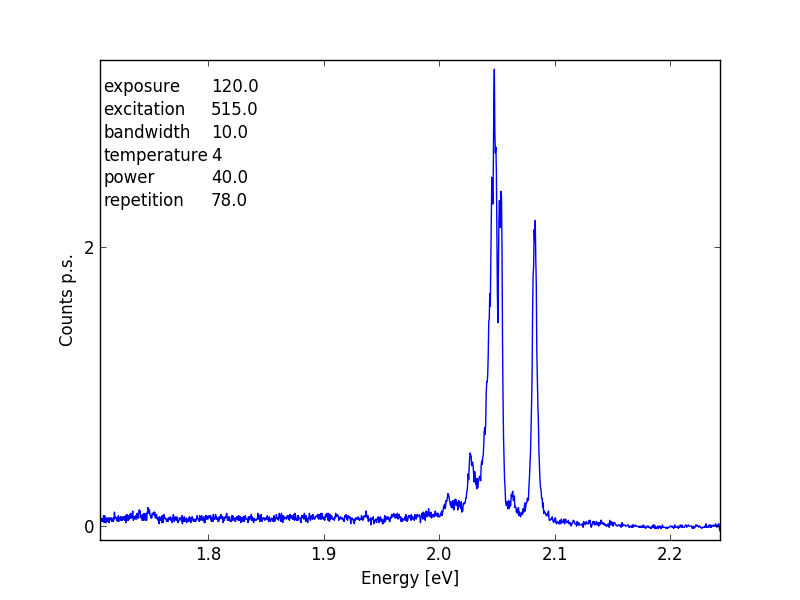
\includegraphics[width=0.45\textwidth]{WL-SCAN-02-hbn-WS2-hbn-SiO-40uW-515nm+-5nm-WLS-78MHz-120s-x41329y08629.png}
\caption{Filename:WL-SCAN-02-hbn-WS2-hbn-SiO-40uW-515nm+-5nm-WLS-78MHz-120s-x41329y08629.png}
\end{figure}
\begin{figure}[H]
\centering
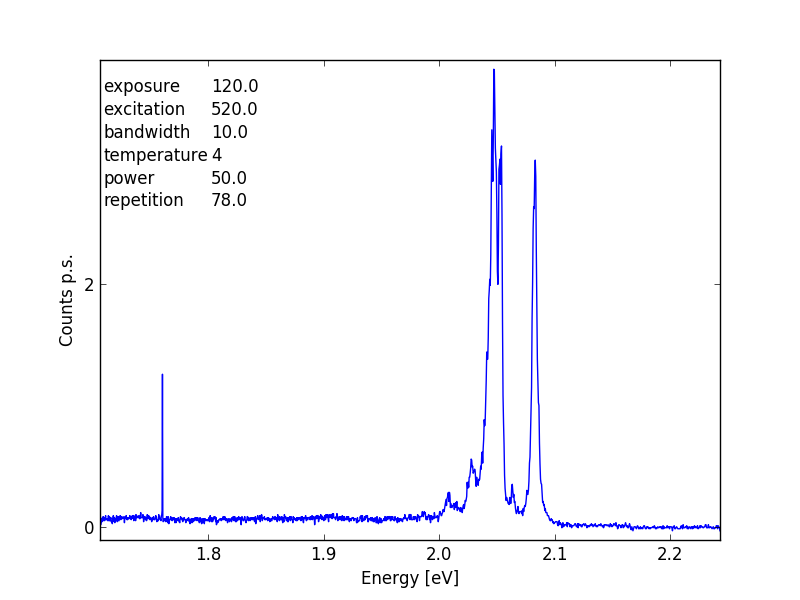
\includegraphics[width=0.45\textwidth]{WL-SCAN-03-hbn-WS2-hbn-SiO-50uW-520nm+-5nm-WLS-78MHz-120s-x41329y08629.png}
\caption{Filename:WL-SCAN-03-hbn-WS2-hbn-SiO-50uW-520nm+-5nm-WLS-78MHz-120s-x41329y08629.png}
\end{figure}
\end{document}
